\documentclass{ccnudoc}

\usepackage{xeCJKfntef, xpinyin}
\usepackage{graphicx}
\usepackage{tabularray}
\usepackage{../exam-zh-choices}
\usepackage{../exam-zh-question}
\usepackage{../exam-zh-symbols}
\usepackage{../exam-zh-chinese}

\ExplSyntaxOn
\NewDocumentCommand \examsetup { m }
  { \keys_set:nn { exam-zh } {#1} }
\ExplSyntaxOff
% \usepackage[
%   backend = biber,
%   style = gb7714-2015
% ]{biblatex}
% \addbibresource{exam-zh.bib}
\graphicspath{{figures}}

\hypersetup{
  pdftitle  = {exam-zh: 高考试卷 LaTeX 模板},
  pdfauthor = {夏康玮}
}
% 全角标点放在引号中,需要改成半角式,否则间距过大,不好看
\def\FSID{“{\xeCJKsetup{PunctStyle=banjiao}。}”} % U+3002
\def\FSFW{“{\xeCJKsetup{PunctStyle=banjiao}.}”} % U+FF0E
\def\COFW{“{\xeCJKsetup{PunctStyle=banjiao}:}”} % U+FF1A
\def\SCFW{“{\xeCJKsetup{PunctStyle=banjiao};}”} % U+FF1B


\title{\textcolor{MaterialIndigo800}{%
  \textbf{exam-zh: 高考试卷 \LaTeX \xpinyin[font=\sffamily,format=\color{MaterialIndigo800}]{模}{mu2}板}}}
\author{李泽平,夏康玮,郭李军}
\date{2022/07/26\quad v0.1.12%
  \thanks{%
    \url{https://gitee.com/zepinglee/exam-zh}
  }
}

\ExplSyntaxOn
\NewDocumentCommand \eu { } { \mathrm{ e } }
\NewDocumentCommand \iu { } { \mathrm{ i } }
\NewDocumentCommand { \scoringbox } { s }
  {
    \IfBooleanTF {#1}
      { \__examzh_scoringbox_onecolumn: }
      { \__examzh_scoringbox_twocolumn: }
  }
\cs_new_protected:Nn \__examzh_scoringbox_twocolumn:
  {
    \begin{tabular}{|c|c|}
      \hline 
      得分 & \rule{3em}{0pt}\rule[-0.7em]{0pt}{2em} \\\hline
      阅卷人 & \rule{3em}{0pt}\rule[-0.7em]{0pt}{2em} \\\hline
    \end{tabular}
  }
\cs_new_protected:Nn \__examzh_scoringbox_onecolumn:
  {
    \begin{tabular}{|c|}
      \hline 
      得分\rule[-0.7em]{0pt}{2em} \\\hline
      \rule[-0.7em]{0pt}{2em} \\\hline
    \end{tabular}
  }
\ExplSyntaxOff


\begin{document}

% 封面的页边距

\newgeometry{
  left   = 2.2 in,
  right  = 1.25 in,
  top    = 1.25 in,
  bottom = 1.00 in
}

\maketitle

% !TeX root = ../exam-zh.tex

\begin{abstract}
  本项目提供了一个中国高考试卷样式的 \LaTeX 模板,旨在帮助中小学教师更方便地使用 \LaTeX。模板具有以下特性:
  
  \begin{enumerate}
    \item 样式与内容尽可能分离;
    \item 选择题选项可以自动排版成合适的列数;
    \item 在 Windows, macOS 和 Linux 跨平台编译。
  \end{enumerate}
\end{abstract}


\begin{tikzpicture}[remember picture, overlay]
  \node[opacity = 0.1,rotate = 30] at ([shift={(0,0)}]current page text area.center){
    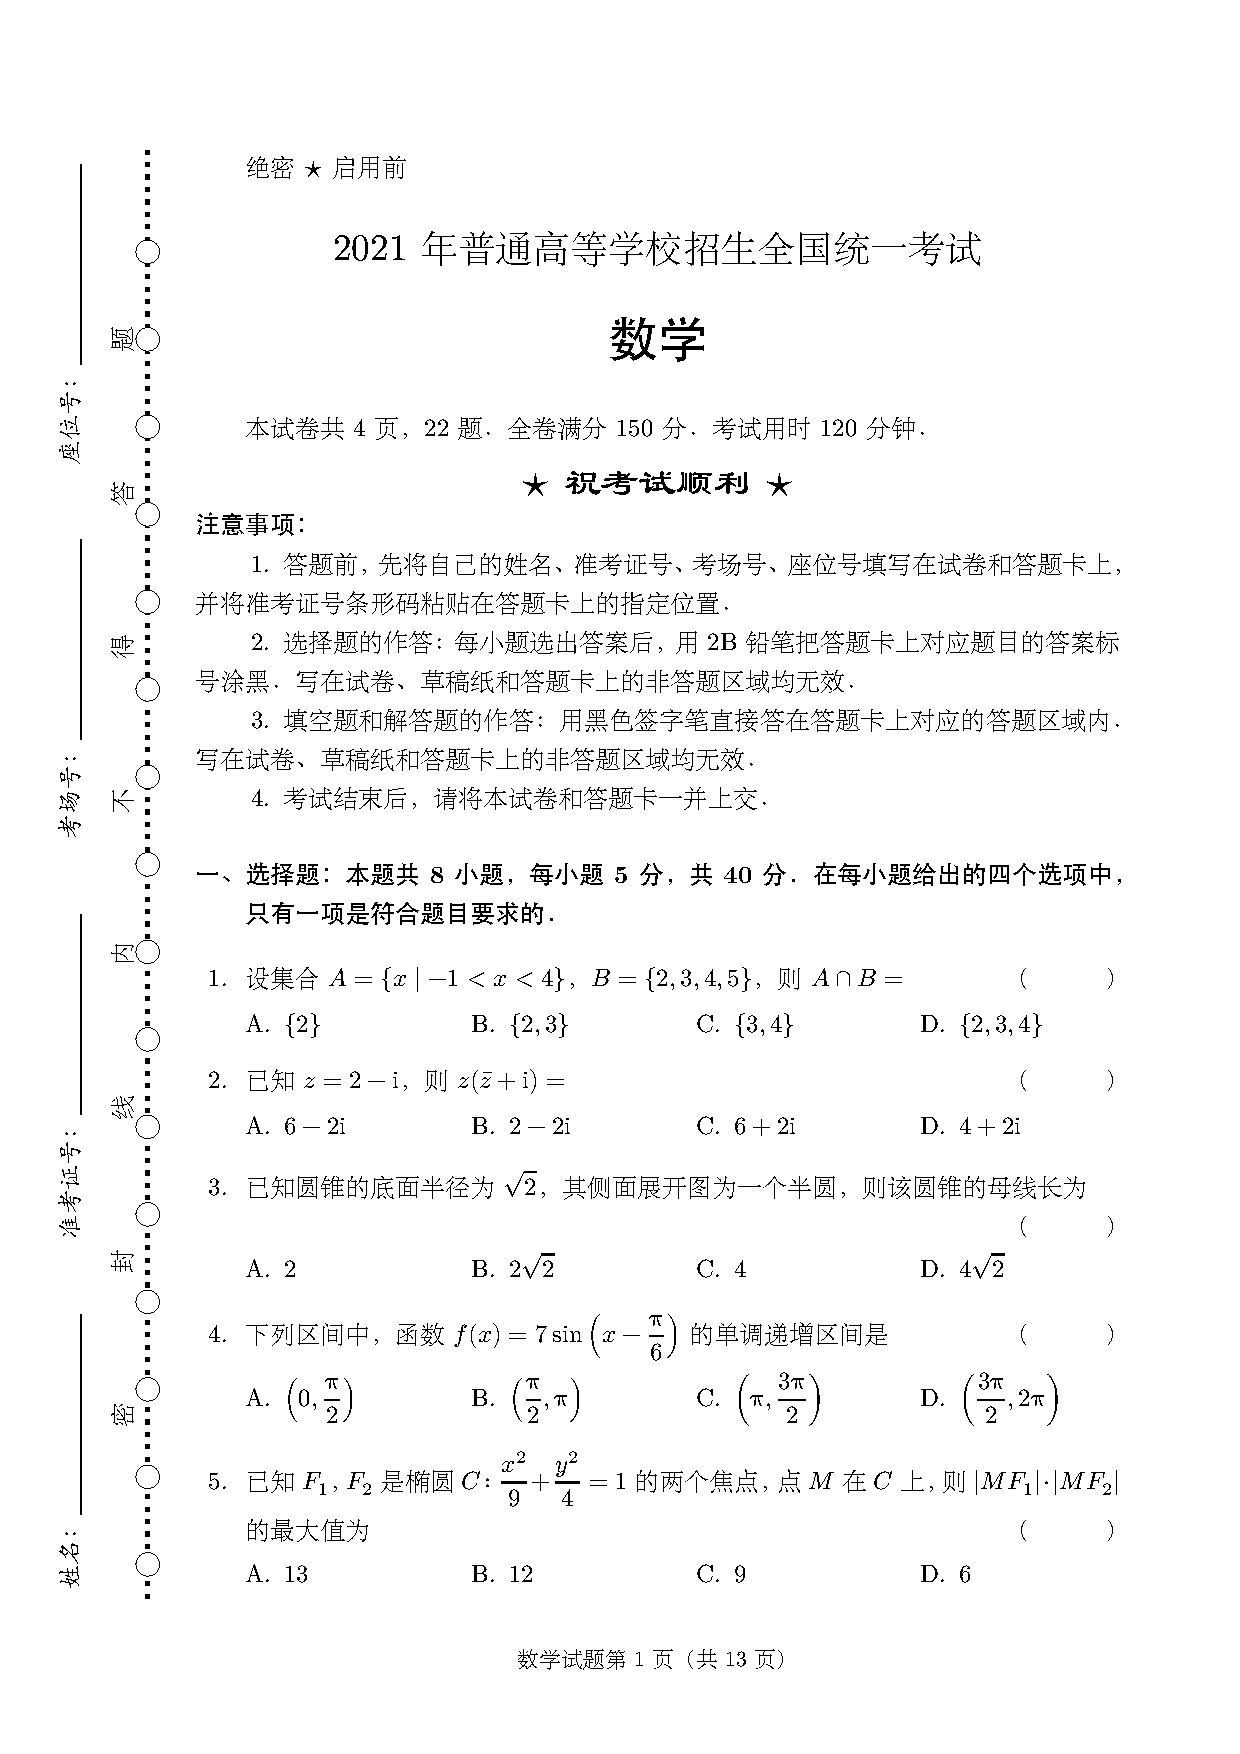
\includegraphics[width=23cm]{firstpage.pdf}
  };
\end{tikzpicture}
\thispagestyle{plain}
\clearpage


% 用户手册的页边距

\newgeometry{
  left   = 1.65 in,
  right  = 0.80 in,
  top    = 1.25 in,
  bottom = 1.00 in
}

\tableofcontents


% 介绍
% !TeX root = ../exam-zh-doc.tex

\section{介绍}

试卷排版是中小学教师经常遇到的需求,目前在网上可以找到的试卷排版相关文类或宏包有:
\begin{itemize}
  \item Philip Hirschhorn:\href{https://www.ctan.org/pkg/exam}{exam}
  \item 吕荐瑞:\href{https://www.ctan.org/pkg/jnuexam}{jnuexam}
  \item 胡振震:\href{https://github.com/hushidong/simplexam}{simplexam}
  \item 鲍宏昌:\href{https://github.com/mathedu4all/bhcexam}{BHCexam}
  \item htharoldht:\href{https://github.com/htharoldht/USTBExam}{USTBExam}
  \item 唐绍东:\href{https://github.com/shaodongtang/gaokao_exam}{GEEexam}
  \item 唐绍东:\href{https://github.com/shaodongtang/CMC}{CMC}
  \item sd44:\href{https://github.com/sd44/DANexam}{DANexam}
\end{itemize}

但是大部分没有经过系统设计以及后续进一步的维护,\href{https://www.ctan.org/pkg/exam}{exam} 大部分设置与国内习惯不同,调试配置起来增加用户的使用成本 \href{https://www.ctan.org/pkg/jnuexam}{jnuexam}、\href{https://github.com/shaodongtang/CMC}{CMC} 是比较“定制化”的,也无法顺利地进行迁移使用。

但是上述前人所做的工作值得参考,比如 \cls{exam-zh} 的 A4 和 A3 页面切换就参考了 \href{https://www.ctan.org/pkg/jnuexam}{jnuexam} 项目。

本模板将借鉴前辈经验,重新设计,并使用 \LaTeX3 编写,以适应 \TeX 技术发展潮流; 同时还将构建一套简洁的接口,方便用户使用。

如果您觉得 \cls{exam-zh} 对您有帮助,也欢迎进行打赏,这会激励维护者更好地维护和开发 \cls{exam-zh}。

\begin{center}
  
\includegraphics[width = 0.7\textwidth]{xdyy-qrcode.png}
\end{center}
% 安装
% % !TeX root = ../exam-zh-doc.tex

\section{安装}

\subsection{获取 \cls{exam-zh}}

目前模块还处于开发阶段,用户目前以「下载发行版」的方式获取最新版本的 \cls{exam-zh}:

\begin{enumerate}
  \item 进入项目主页(\href{https://gitee.com/zepinglee/exam-zh}{gitee 项目主页} (界面见图~\ref{figure:gitee项目主页} )
  \item 在右侧一列有“发行版”(gitee),并且有一个标签图标并有“vx.x.x - 20xx-xx-xx”字样,表示最新的发行版版本和发布时间,点击即可查看相关信息(如果想查看历史所有发行版信息,可以点击“发行版”右侧的“全部”(gitee))。
  
    发行版中一般由以下信息构成(\href{https://gitee.com/zepinglee/exam-zh/releases}{gitee 发行版} 界面见图~\ref{figure:gitee发行版})
      \begin{itemize}
        \item 更新文件的特别说明。如果没有,则表明此次更新只需要更新 \file{exam-zh.cls} 文件至最新\footnote{“更新 \meta{文件} 至最新”目前表示在发行版中下载最新版本的模板,并用其中所需要更新的 \meta{文件} 去替换本地的旧 \meta{文件}} 即可
        \item 更新日志。 主要为此次发行版与上次发行版的不同,一般为“Added”、“Changed”、“Fixed”等信息
        \item 模版及用户手册下载链接(“下载”部分)。一般用户只需要点击 \file{exam-zh-vx.x.x.zip} 进行模版下载即可,而下面的 \file{Source code} 为项目的整个源码,包括手册的源码,测试文件等,如果感兴趣的用户可以下载进行查看(当然,如果会使用 \cmd{git} 的用户也可以将整个 \cls{exam-zh} 项目 \cmd{clone} 下来查看)
      \end{itemize}
  \item 点击 \file{exam-zh-vx.x.x.zip} 进行下载,在本地解压即可
\end{enumerate}


\begin{figure}[htbp]
  \centering
  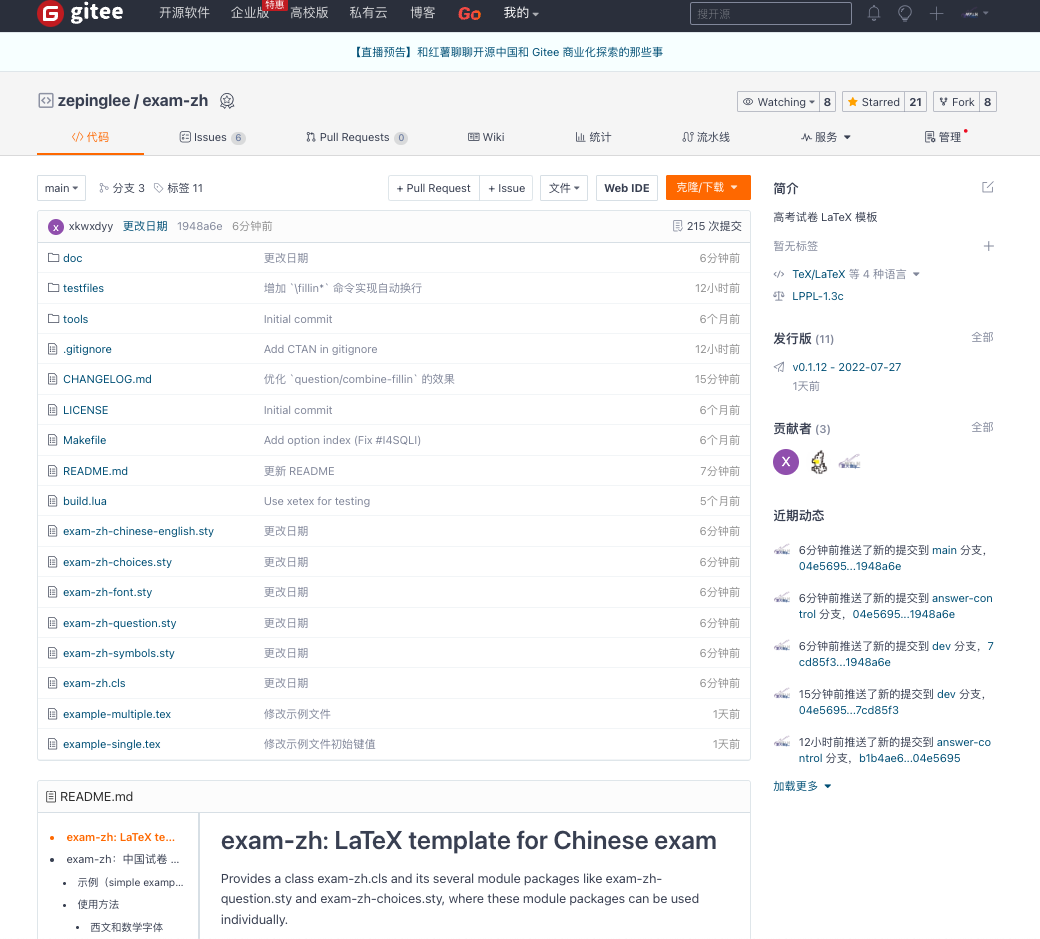
\includegraphics[width = \textwidth]{gitee-main.png}
  \caption{gitee 项目主页}
  \label{figure:gitee项目主页}
\end{figure}


\begin{figure}[htbp]
  \centering
  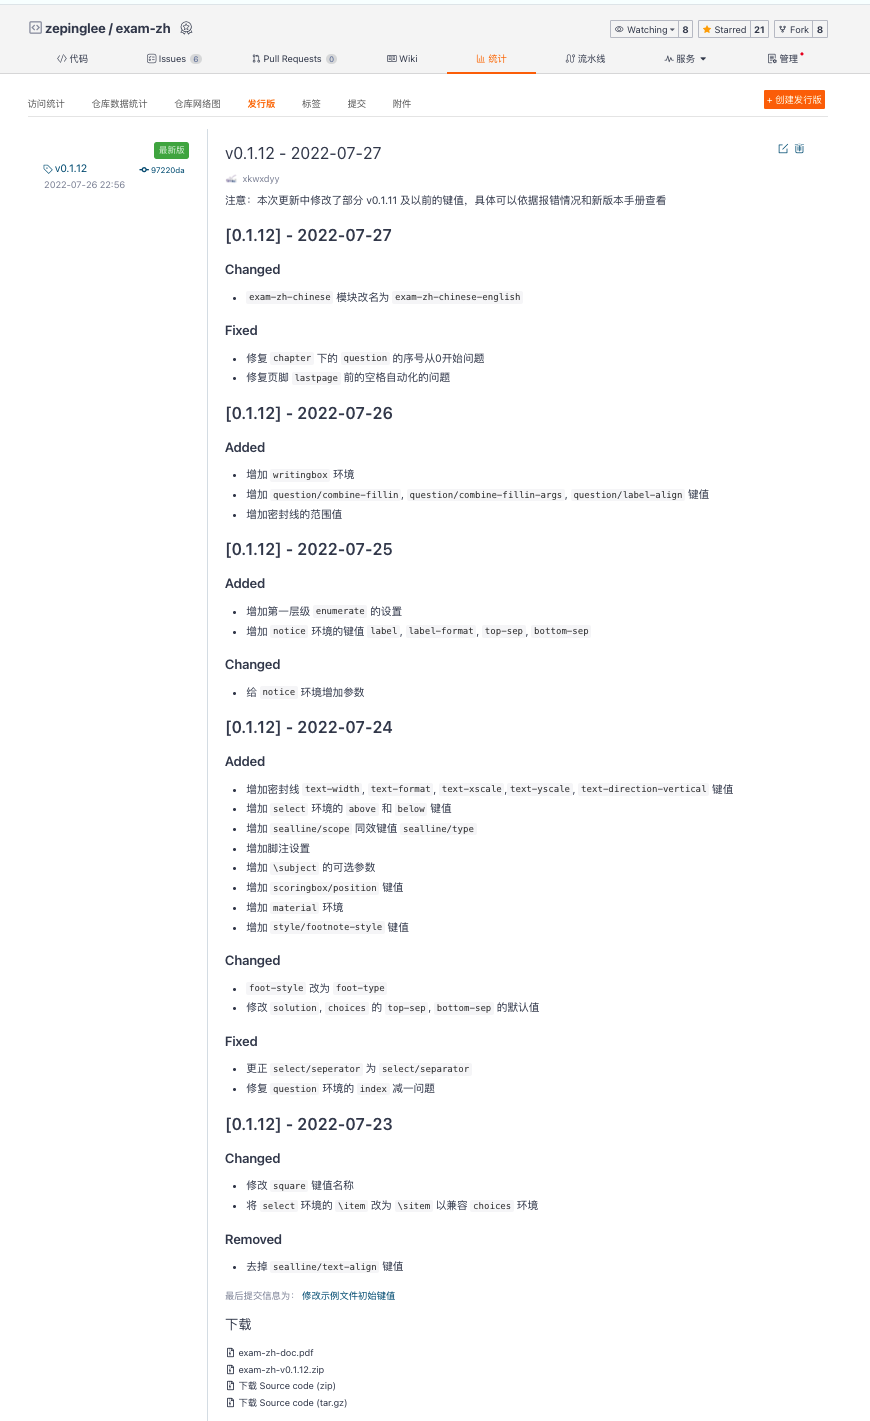
\includegraphics[width = \textwidth]{gitee-release.png}
  \caption{gitee 发行版}
  \label{figure:gitee发行版}
\end{figure}

% % \subsubsection{标准安装}

% % 如果没有特殊理由,始终建议您使用宏包管理器安装 \cls{exam-zh}。
% % 例如在 \TeXLive{} 中,执行(可能需要管理员权限)
% % \begin{shellexample}[morekeywords={tlmgr,install}]
% %   tlmgr install exam-zh
% % \end{shellexample}
% % 即可完成安装。

% % 在 \TeXLive{} 和 \MiKTeX{} 中,您还可以通过图形界面进行安装,
% % 此处不再赘述。

% % \subsubsection{手动安装}

% % 如果您需要从 CTAN 上自行下载并手动安装,较好的方法是使用 TDS
% % 安装包:
% % \begin{itemize}
% %   \item 从 CTAN 上下载 \cls{exam-zh} 的
% %     \href{http://mirror.ctan.org/install/macros/latex/contrib/exam-zh.tds.zip}{TDS 安装包};
% %   \item 按目录结构将 \file{exam-zh.tds.zip} 中的文件复制到 \TeX{}
% %     发行版的本地 TDS 根目录;
% %   \item 执行 \bashcmd{mktexlsr} 刷新文件名数据库以完成安装。
% % \end{itemize}
% % %
% % 您也可以从源代码直接生成模板(不推荐):
% % \begin{itemize}
% %   \item 打开 \href{https://gitee.com/stone-zeng/exam-zh}{项目主页},
% %     点击“Code”按钮,并选择“Download ZIP”,下载 \file{exam-zh-main.zip};
% %     如果您的电脑中安装有 git 程序,也可通过以下命令直接克隆代码仓库:
% %     \begin{shellexample}[gobble=6,alsoletter={.},morekeywords={git,clone}]
% %       git clone https://gitee.com/stone-zeng/exam-zh.git
% %     \end{shellexample}
% %   \item 解压并进入到 \file{source} 文件夹,执行以下命令以生成
% %     模板的各组件:
% %     \begin{shellexample}[gobble=6,morekeywords={xetex}]
% %       xetex exam-zh.dtx
% %     \end{shellexample}
% %   \item 将生成的文档类(\file{.cls})、宏包(\file{.sty})以及
% %     参数配置文件(\file{.def})复制到 \TeX{} 发行版本地 TDS 树
% %     的 \path{texmf-local/tex/latex/exam-zh/} 目录下,并执行
% %     \bashcmd{mktexlsr} 刷新文件名数据库,方可完成安装。
% %   \item 使用 \cls{exam-zh} 撰写论文时,您还需要从代码仓库下的
% %     \file{testfiles/support} 目录中复制 \file{fudan-name.pdf}
% %     文件至工作目录,以确保封面中的校名图片可以正确显示。
% % \end{itemize}

% % \subsubsection{扁平化安装}

% % 如果您不希望安装本模板,但需要立刻使用,也可以使用模板提供的安装脚本。
% % 从 gitee 上获取代码仓库后,执行 \file{install-win.bat}(Windows 系统)
% % 或 \file{install-linux.sh}(Linux 系统),所有需要的文件便会在
% % \file{thesis} 文件夹中生成。


\subsection{模板组成}

本模板主要包含核心文档类、参考文献格式文件以及用户文档等几个部分,
其具体组成见表~\ref{tab:exam-zh-main-components}。

\begin{table}[htbp]
  \caption{\cls{exam-zh} 的主要组成部分}
  \label{tab:exam-zh-main-components}
  \centering
  \small
  \begin{tblr}{
    hline{1, 2, Z} = {1pt},
    width = \textwidth,
    colspec = {X[3,l]X[5.5,l]},
    rows = {m}
  }
    \textbf{文件} & \textbf{功能说明} \\
    \file{exam-zh-doc.pdf}            & 用户手册(本文档) \\
    \file{example-single.tex}、\file{example-multiple.tex}            & 模板的主文件(同时也是示例文件),可据此为基础完成试卷编写 \\
    \file{exam-zh.cls}            & 模板文档类 \\
    \file{exam-zh-choices.sty}    & 模版的选择题模块宏包\\
    \file{exam-zh-question.sty}   & 模版的题干模块宏包\\
    \file{exam-zh-font.sty}       & 模版的字体模块宏包\\
    \file{exam-zh-symbols.sty}    & 模版的符号模块宏包\\
    \file{exam-zh-chinese-english.sty}    & 模版的语文英语模块宏包\\
    \file{README.md}              & 简要自述 \\
    \file{CHANGELOG.md}           & 模板更新日志 \\
    \file{LICENSE}                & 模版发布许可证
  \end{tblr}
\end{table}

% \begin{table}[htbp]
%   \caption{\cls{exam-zh} 各目录的组成部分}
%   \label{tab:exam-zh-sub-components}
%   \centering
%   \small
%   \begin{tblr}{
%     hline{4,5,8,11,13} = {solid},
%     hline{1, 2, Z} = {1pt},
%     width = \textwidth,
%     colspec = {X[1,l]X[3,l]X[3,l]},
%     rows = {m},
%     cell{2}{1} = {r=2}{m},
%     cell{5}{1} = {r=3}{m},
%     cell{8}{1} = {r=3}{m},
%     cell{11}{1} = {r=2}{m},
%   }
%     \textbf{子目录} & \textbf{子目录中的文件} & \textbf{功能说明} \\
%     front & \file{abstract.tex}            & 中英文摘要 \\
%     front & \file{notation.tex}            & 符号表 \\
%     body  & \file{chapter<number>.tex}     & 正文的分文件 \\
%     back  & \file{acknowledgements.tex}    & 致谢 \\
%     back  & \file{appendix.tex}            & 附录 \\
%     back  & \file{publications.tex}        & 攻读学位期间取得的研究成果(博士)\\
%     logo  & \file{ccnulogo.png}            & “华中师范大学”字样 logo \\
%     logo  & \file{masterlogo.png}          & 硕士学位论文页眉 logo \\
%     logo  & \file{doctorlogo.png}          & 博士学位论文页眉 logo \\
%     copyright  & \file{Originality_Copyright.pdf}  & 本科学位论文原创性声明和使用授权说明 \\
%     copyright  & \file{Originality_Copyright_master_doctor.pdf}  & 硕博学位论文原创性声明和使用授权说明\\
%     figures & & 用户放置图片的目录\\
%   \end{tblr}
% \end{table}



% 参与开发
% % !TeX root = ../exam-zh.tex

\section{参与开发}

\begin{itemize}
  \item 如果您有任何改进意见或者功能需求,欢迎前往 \href{https://gitee.com/zepinglee/exam-zh/issues}{gitee 仓库 issues} 提交 issue
  \item 欢迎 \cmd{fork} 本项目,提 \cmd{pr} 的形式参与开发
  \item 建议阅读 \href{https://zhuanlan.zhihu.com/typography-and-latex/}{muzimuzhi} 写的 \href{https://gitee.com/ustctug/ustcthesis/wiki/%E5%8F%82%E4%B8%8E%E5%BC%80%E5%8F%91}{参与开发}
  \item 参考阅读
    \begin{itemize}
      \item \href{https://www.zhihu.com/question/27017364/answer/34932199}{知乎:开发一个 LaTeX 宏包需要多少知识?}
      \item \href{https://zhuanlan.zhihu.com/p/19669122}{The TeXbook 导读:从那头(多图杀猫的)狮子说起}
    \end{itemize}
\end{itemize}



% 关于作者
% % !TeX root = ../exam-zh.tex

\section{关于模版作者和维护者}

\href{https://github.com/zepinglee}{zepinglee} 开发了模版前期的大框架和主要功能(\file{exam-zh-choices.sty}、\file{exam-zh-question.sty}、\file{exam-zh-font.sty} 等)。

\href{https://github.com/xkwxdyy}{xkwxdyy} 和 \href{https://github.com/ljguo1020}{ljguo} 为模版的后期维护者。

非常感谢 \href{https://github.com/syvshc}{syvshc} 在开发中提供的帮助!



\section{TODO}

\begin{itemize}
  \item 密封线的格子连续排版
  \item 学生信息在顶部的设计(参考2022年高考)
  \item 设计接口
    \begin{itemize}
      \item 页脚内容
      \item 标题
      \item 科目的显示
      \item \tn{goodluck} 的显示
    \end{itemize}
  \item 答案控制
\end{itemize}

% 参考文献
% \printbibliography



\end{document}